
\section{Online-PCA}

\mode<presentation>{
\begin{frame} 
    \begin{center} \huge
        \secname
    \end{center}
\end{frame}
}

\begin{frame}
W\notesonly{e have established that w}e can use Hebbian learning (Oja's rule to prevent divergence) 
to find the direction of the first \notesonly{principle component $\vec e_1$}\slidesonly{PC} in the data. \\

\pause

Note that
\begin{align}\text{with} \quad \vec w &= \vec e_1\\
\text{follows} \quad y &= \vec e_1^\top \vec x =: a_1
\end{align}

\question{What else is there to do?}

\pause

- All other PCs

\end{frame}

\begin{frame}{Only}\frametitle{\secname}
%\only<1>{
\svspace{-5mm}
\begin{center}
%\includegraphics<1>[width=4cm]{img/section2_fig5_b_2}
%\slidesonly{
%\includegraphics<2>[width=4cm]{img/section2_fig5_b_2_blue}
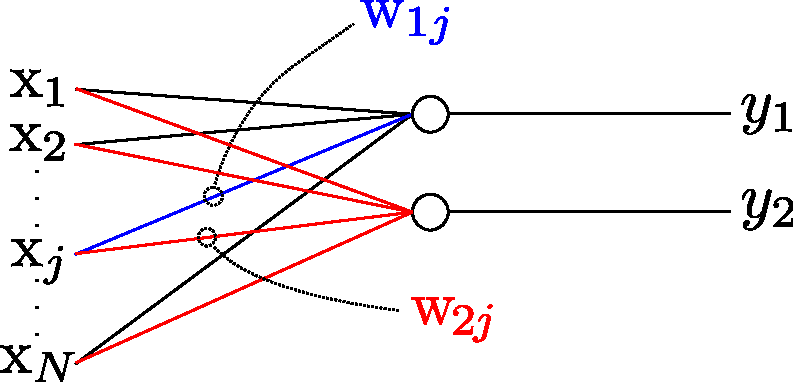
\includegraphics[width=4cm]{img/section2_fig5_b_2_blue-red}
%}
\captionof{figure}{A neural network}
\end{center}
\svspace{-3mm}

\only<1>{
We proceed to learning the next PC by doing the following:
}
\begin{enumerate}
\item<only@1> Denote the network's response with $y_1$ and its weight vector as $\color{blue}\vec w_1$, knowing that ${\color{blue}\vec w_1} = \vec e_1$.
\item<only@1> Add a second neuron $y_2$ to our network. This neuron will come with its own randomly initialized weight vector $\color{red}\vec w_2$.
\item<only@1,2> Resume feeding new data points into the network computing its response $y_1$ and $y_2$.
\item<only@2,3> We exploit that the PCs form an \emph{orthonormal basis}, specifically, we obtain a projection of $\vec x$ 
into the subspace orthogonal to $\vec e_1$\notesonly{ that is the first PC}:
\begin{align}
\hat x_j &= x_j - {\color{blue} w_{1j}} \, y_1 \only<2>{
\intertext{Recall: ${\color{blue}\vec w_1} = \vec e_1 \rightarrow \; y = \vec e_1^\top \vec x =: a_1$}}
         \only<2>{&}= x_j - a_1 (\vec e_1)_j
         \label{eq:projorth}
\end{align}

%\slidesonly{
%\only<2>{
%\placeimage{11}{7}{img/section2_fig5_b_2_blue}{width=4cm}
%}
%\only<3>{
%\placeimage{11}{7}{img/section2_fig5_b_2_blue-red}{width=4cm}
%}
%}
\notesonly{where $\color{blue}w_{1j}$ is the weight of the connection between $\hat x_j$ and the neuron $y_1$,}
\item<only@3-> Apply Oja's rule on $\color{red}\vec w_2$.

For \underline{stationary} data: No need to apply updates to $\color{blue}\vec w_1$ anymore, since it has already converged to $\vec e_1$.\notesonly{ Applying the update to $\color{blue}\vec w_1$ would only yield negligible change in the case of stationary data.}
\slidesonly{Further updates would lead to negligible change.}
 
\item<only@3-> Continue feeding observations until $\color{red}\vec w_2$ has converged.
\item<only@3-> On convergence, ${\color{red}\vec w_2} = \vec e_2$.
\end{enumerate}

\end{frame}

\begin{frame}


\begin{center}
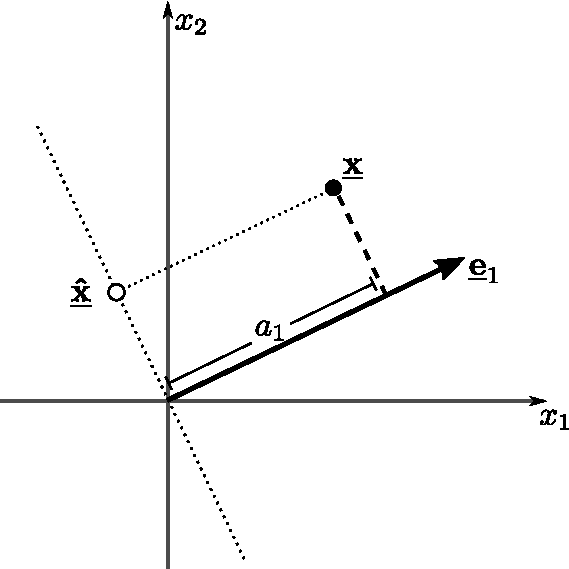
\includegraphics[width=4cm]{img/othogonality_novelty_less}
\captionof{figure}{A graphical interpretation}
\end{center}

\notesonly{\label{eq:projorth} }using vector notation:
\begin{align}
\hat {\vec x} &= \vec x - \vec w_1 \, y_1\\
			&= \vec x - a_1 \vec e_1
\end{align}

\pause

We get the remaining PCs by repeating the above except, that we project 
the data onto the subspace orthogonal to \textbf{all previous} PCs.\\
(cf. lecture slides 1.2 ``Learning: Oja's rule \& Gram-Schmidt orthonormalization'')

\end{frame}

